\documentclass[aspectratio=169]{beamer}

\usepackage[T1]{fontenc}
\usepackage[english]{babel}
\usepackage[utf8]{inputenc}
\usepackage{todonotes}
\usepackage{subfig}
\usepackage{tikz}
\usepackage[round]{natbib}
\usepackage{booktabs,multirow}
\usepackage{adjustbox}
\usepackage{comment}
\usepackage[normalem]{ulem}

\usepackage{amsmath,amsfonts,amssymb}

\usepackage{caption}
\captionsetup[figure]{labelformat=empty}

\usepackage{algpseudocode}
\usepackage[linesnumbered,ruled]{algorithm2e}
\SetArgSty{textnormal}
\DontPrintSemicolon

\usetikzlibrary{arrows,shapes,mindmap,backgrounds}

% Declare layers
\pgfdeclarelayer{background}
\pgfsetlayers{background,main}

% Easier TO-DO notes
\newcommand{\Todo}[1]{\todo[inline]{\scriptsize #1}}

% 1: Slide number
% 2: Highlight color
% 3: Text to be formatted
\newcommand{\onlyh}[3]{
   \only<#1> {\color{#2}}
   #3
   \only<#1> {\normalcolor}
}

\usetheme{Inf}

\title[EURO 2021H -- Solving daily-HHCRSP with route interdependencies]
      {Solving the single-day home health care problem with route interdependencies}

% Optional subtitle
\subtitle{EURO 2021H --- MD-35}

\date{July 12, 2021}

% Author information
\author{\footnotesize Alberto F. Kummer, Olinto C.B. de Araújo, Luciana S. Buriol, and Mauricio G.C. Resende}

\institute{Institute of Informatics --- UFRGS\\\texttt{\{afkneto,buriol\}@inf.ufrgs.br}}

% Commands to help writing the presentation.
\newcommand{\C}{\mathcal{C}}
\newcommand{\Cz}{\C^0}
\newcommand{\Cs}{\C^\mathrm{s}}
\newcommand{\Cd}{\C^\mathrm{d}}
\newcommand{\Sk}{\mathcal{S}}
\newcommand{\dmin}{\delta^\mathrm{min}}
\newcommand{\dmax}{\delta^\mathrm{max}}
\newcommand{\V}{\mathcal{V}}

\begin{document}

% Command to create title page
\InfTitlePage

\begin{frame}
  \frametitle{Outline}
  \tableofcontents
\end{frame}
%
%\section{Blocos}

%\begin{frame}[plain]
% \sectionpage
%\end{frame}

\section{Introduction}

\begin{frame}[plain]
   \sectionpage
\end{frame}

\frame{
   \frametitle{Logistic management for healthcare systems}

   \textbf{Overview of HHCP}
   \begin{itemize}
      \item First study from \citeyear{fernandez1974}
      \item Home care: patients receive healthcare in their \emph{homes}
      \item Traditional systems: patients receive healthcare in \emph{hospitals}
   \end{itemize}

   \vspace*{18pt}

   \begin{figure}[H]
      \centering
      
\includegraphics[scale=0.15]{fig/fernandez-paper.png}
   \end{figure}
}

\frame{
   \frametitle{Logistic management for healthcare systems}

   \textbf{Ease the access to health and social care services}
   \begin{itemize}
      \item More inclusive
      \item Alternative to nursing homes
      \item Leverage hospital beds for complex cases
   \end{itemize}

   \vspace*{12pt}

   \textbf{Arriving challenge:} Efficient routing solution for caregivers to patient locations.
}

\frame{
   \frametitle{Logistic management for healthcare systems}

   \textbf{Core of home care problems}: A vehicle routing problem with additional constraints.

   \vspace*{12pt}

   \only<+> {
      \begin{figure}[H]
         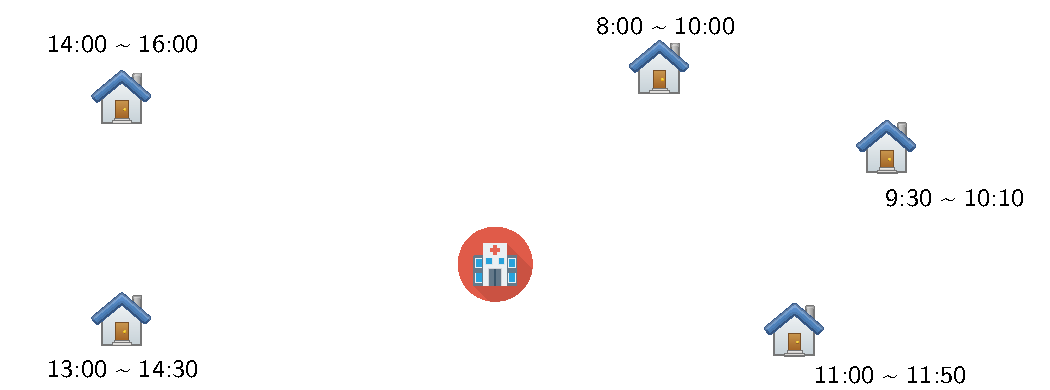
\includegraphics[width=0.8\textwidth, page=1]{fig/routing-example}%
      \end{figure}
   }

%   \only<+> {
%      \begin{figure}[H]
%         \includegraphics[width=0.8\textwidth, page=2]{fig/routing-example}%
%      \end{figure}
%   }
%
%   \only<+> {
%      \begin{figure}[H]
%         \includegraphics[width=0.8\textwidth, page=3]{fig/routing-example}%
%      \end{figure}
%   }
%
%   \only<+> {
%      \begin{figure}[H]
%         \includegraphics[width=0.8\textwidth, page=4]{fig/routing-example}%
%      \end{figure}
%   }
%
%   \only<+> {
%      \begin{figure}[H]
%         \includegraphics[width=0.8\textwidth, page=5]{fig/routing-example}%
%      \end{figure}
%   }

   \only<+> {
      \begin{figure}[H]
         \includegraphics[width=0.8\textwidth, page=6]{fig/routing-example}%
      \end{figure}
   }
}

%\frame{
%   \frametitle{Logistic management for healthcare systems}
%
%   \textbf{Arriving challenge:} Efficient routing solution for caregivers to patient locations.
%
%   \begin{itemize}
%      \item Reduces hospitalization costs
%      \item Decentralized care
%      \item Increases patients comfort
%      \item Reduces patient stress and the pressure of mental health
%   \end{itemize}
%}

\frame{
   \frametitle{Logistic management for healthcare systems}

   \textbf{Increased life expectancy}

   \only<1> {
   \begin{itemize}
      \item Population aging
      \item Exhaustion of public healthcare services
   \end{itemize}
   }


   \only<1,2> {
      \begin{figure}[H]

         \subfloat[Brazil in 2010]{
            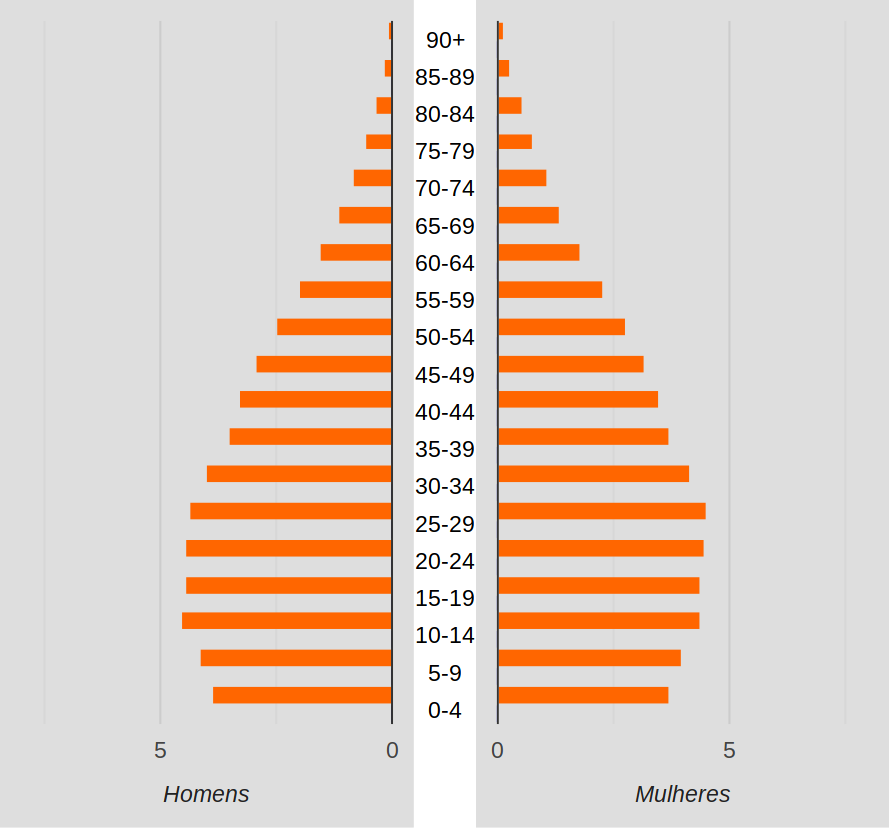
\includegraphics[width=0.25\textwidth]{fig/piramide-2010.png}

         }
         \hfill
         \subfloat[Brazil in 2021]{
           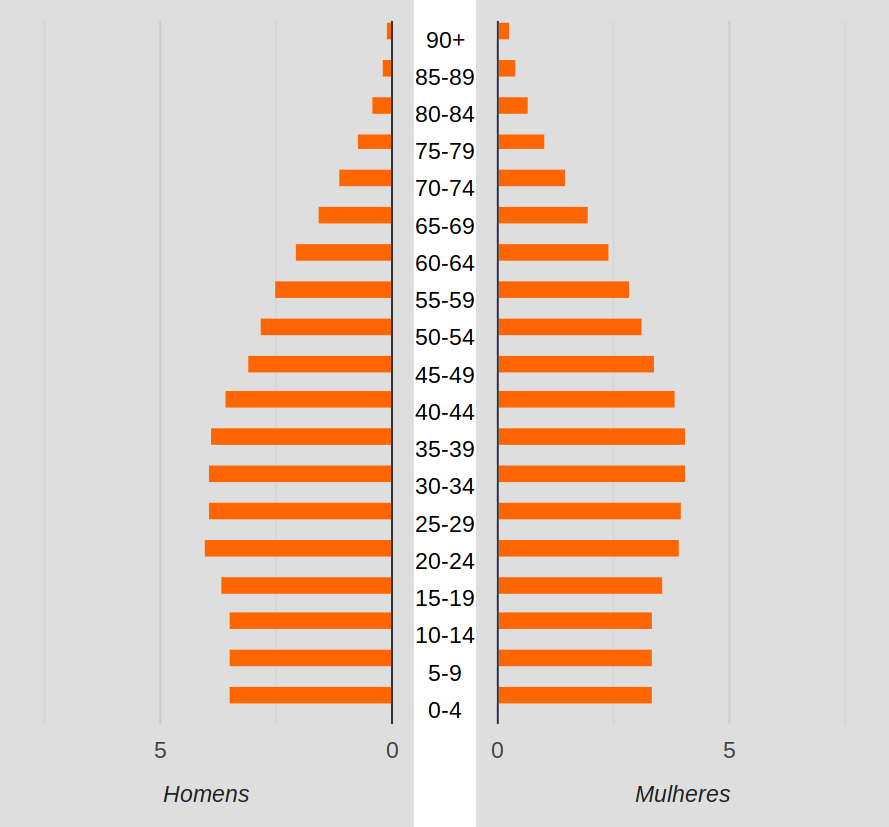
\includegraphics[width=0.25\textwidth]{fig/piramide-2021.png}

         }
         \hfill
         \subfloat[Brazil in 2050]{
            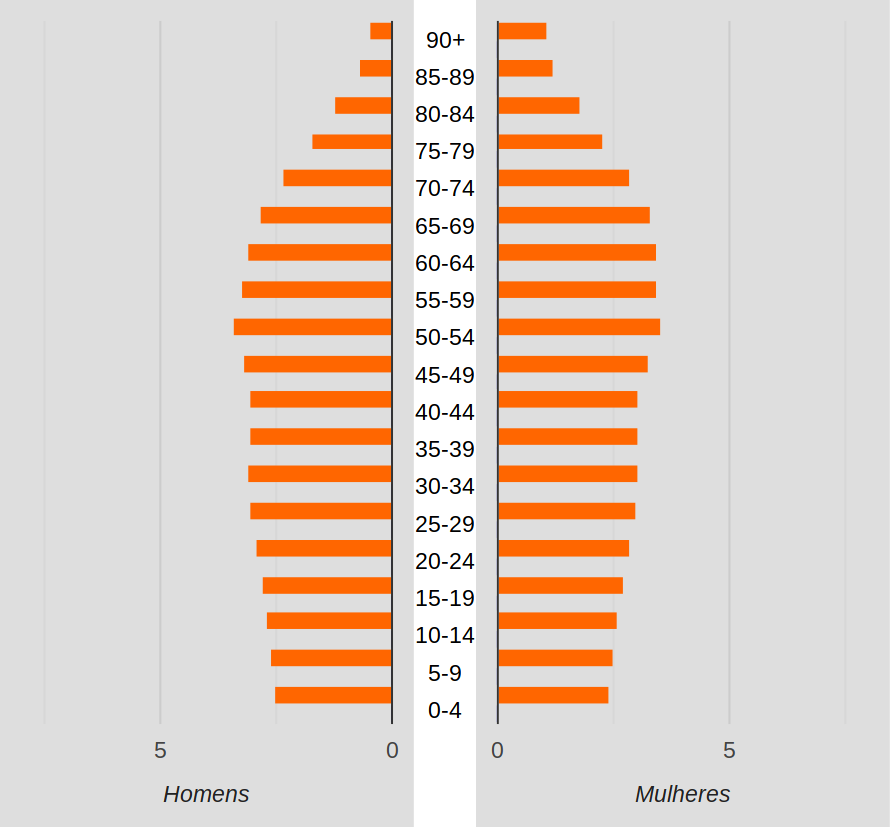
\includegraphics[width=0.25\textwidth]{fig/piramide-2050.png}

         }

         \caption{Source: Brazilian Institute of Geography and Statistics (2010)}

      \end{figure}
   }

   \only<2> {
%      \begin{figure}[H]
%         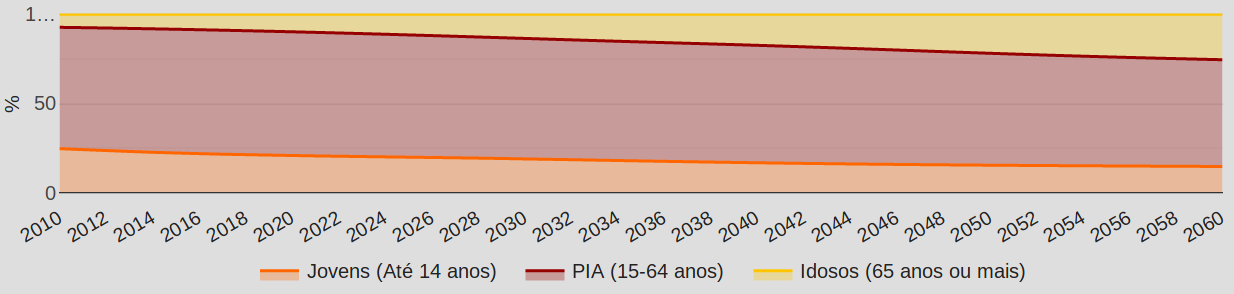
\includegraphics[width=\textwidth]{fig/brazilian-pop-evol.png}
%         \caption{Source: Brazilian Institute of Geography and Statistics (2010)}
%      \end{figure}

%      Estimated population over 65+ years:
      \footnotesize
      \begin{itemize}
         \item In 2010: \phantom{0}7.32\% (14M people)
         \item In 2021: 10.15\% (21M people)
         \item In 2050: \color{InfRed} 21.87\% (51M people)
      \end{itemize}
   }
}


\frame{
   \frametitle{Logistic management for healthcare systems}

%   \begin{tikzpicture}[overlay]
%   \node at (9.5,-0.3) {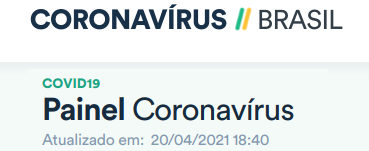
\includegraphics[scale=0.4]{fig/snapshot-covid}} ;
%   \end{tikzpicture}
%
%   \vspace{4pt}

   \textbf{Covid-19 pandemic in Brazil}
   \begin{figure}[H]
      \subfloat[Total cases (\textasciitilde 14M)]{
         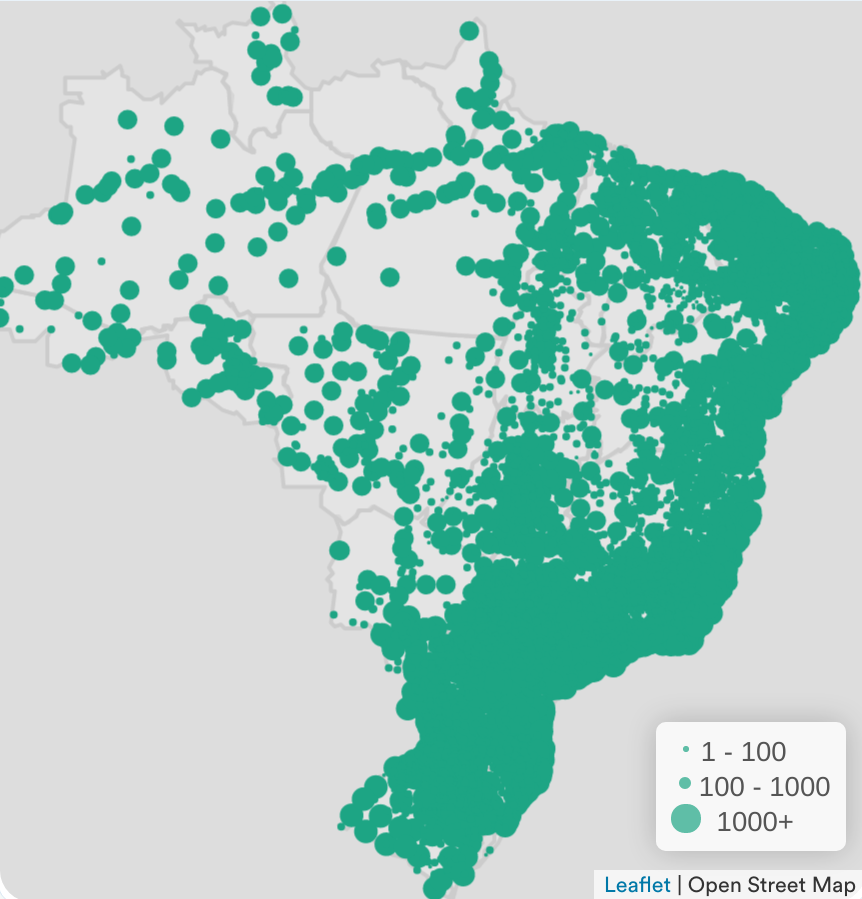
\includegraphics[width=0.3\textwidth]{fig/casos-covid}
      }
      \hspace*{40pt}
      \subfloat[Total deaths (\textasciitilde 378k)]{
         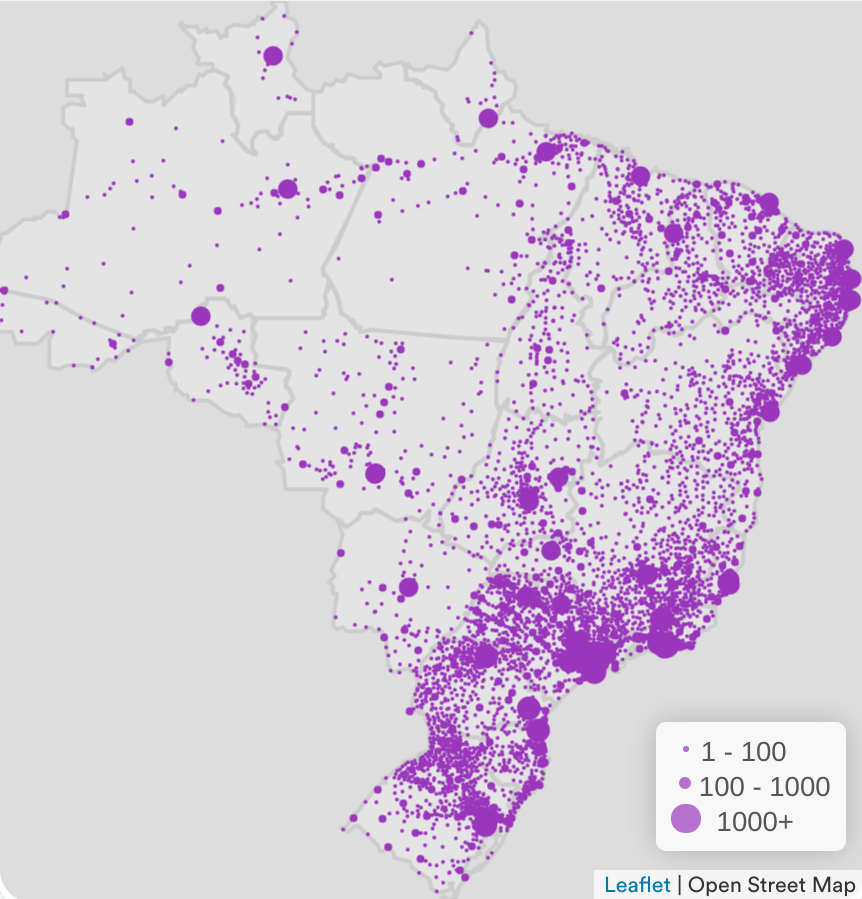
\includegraphics[width=0.3\textwidth]{fig/obitos-covid}
      }
      \caption{Source: DATASUS (2021)}
   \end{figure}
}

\frame{
   \frametitle{Logistic management for healthcare systems}

   \textbf{Covid-19 pandemic in Brazil}
   \begin{itemize}
      \item Lack of testing
      \item Lack of monitoring
   \end{itemize}

   \vspace{12pt}

   \textbf{But our public health system could be doing more}
   \begin{itemize}
      \item \emph{Better in Home}: pilot HHC program
%      \item Before the pandemic: weekly visit by health agents
      \item In Porto Alegre: vaccination through HHC structure
   \end{itemize}
}

\section{Related works}

\begin{frame}[plain]
   \sectionpage
\end{frame}


\frame{
   \frametitle{Literature outline}

   \textbf{In general}
   \begin{itemize}
      \item Most publications approach \emph{only} the routing problem \citep{gutierrez2013,grieco2020}
      \item Three surveys on routing problems arriving HHCP: \citet{fikar2017}, \citet{cisse2017}, and \citet{grieco2020}
      \item This is also the case of this thesis proposal
   \end{itemize}
}

\frame{
   \frametitle{Literature outline}

   \textbf{HHC involves much more than routing and scheduling}
   \begin{itemize}
      \item Placement of operation centers
      \item Choice of health and social services offered
      \item Staffing and supplier selection
      \item Fleet assignment and staff routing
      \item Inventory management
   \end{itemize}

    \vspace*{12pt}

   \textbf{Lots of similarities with supply chain and task workforce problems \citep{ballou2007,castillo2016}}
%   \begin{itemize}
%      \item Strategical planning
%      \item Tactical planning
%      \item Operational planning
%   \end{itemize}
}

\frame{
   \frametitle[plain]{Literature outline}

   \begin{center}
      \begin{adjustbox}{width=0.6\textwidth}

      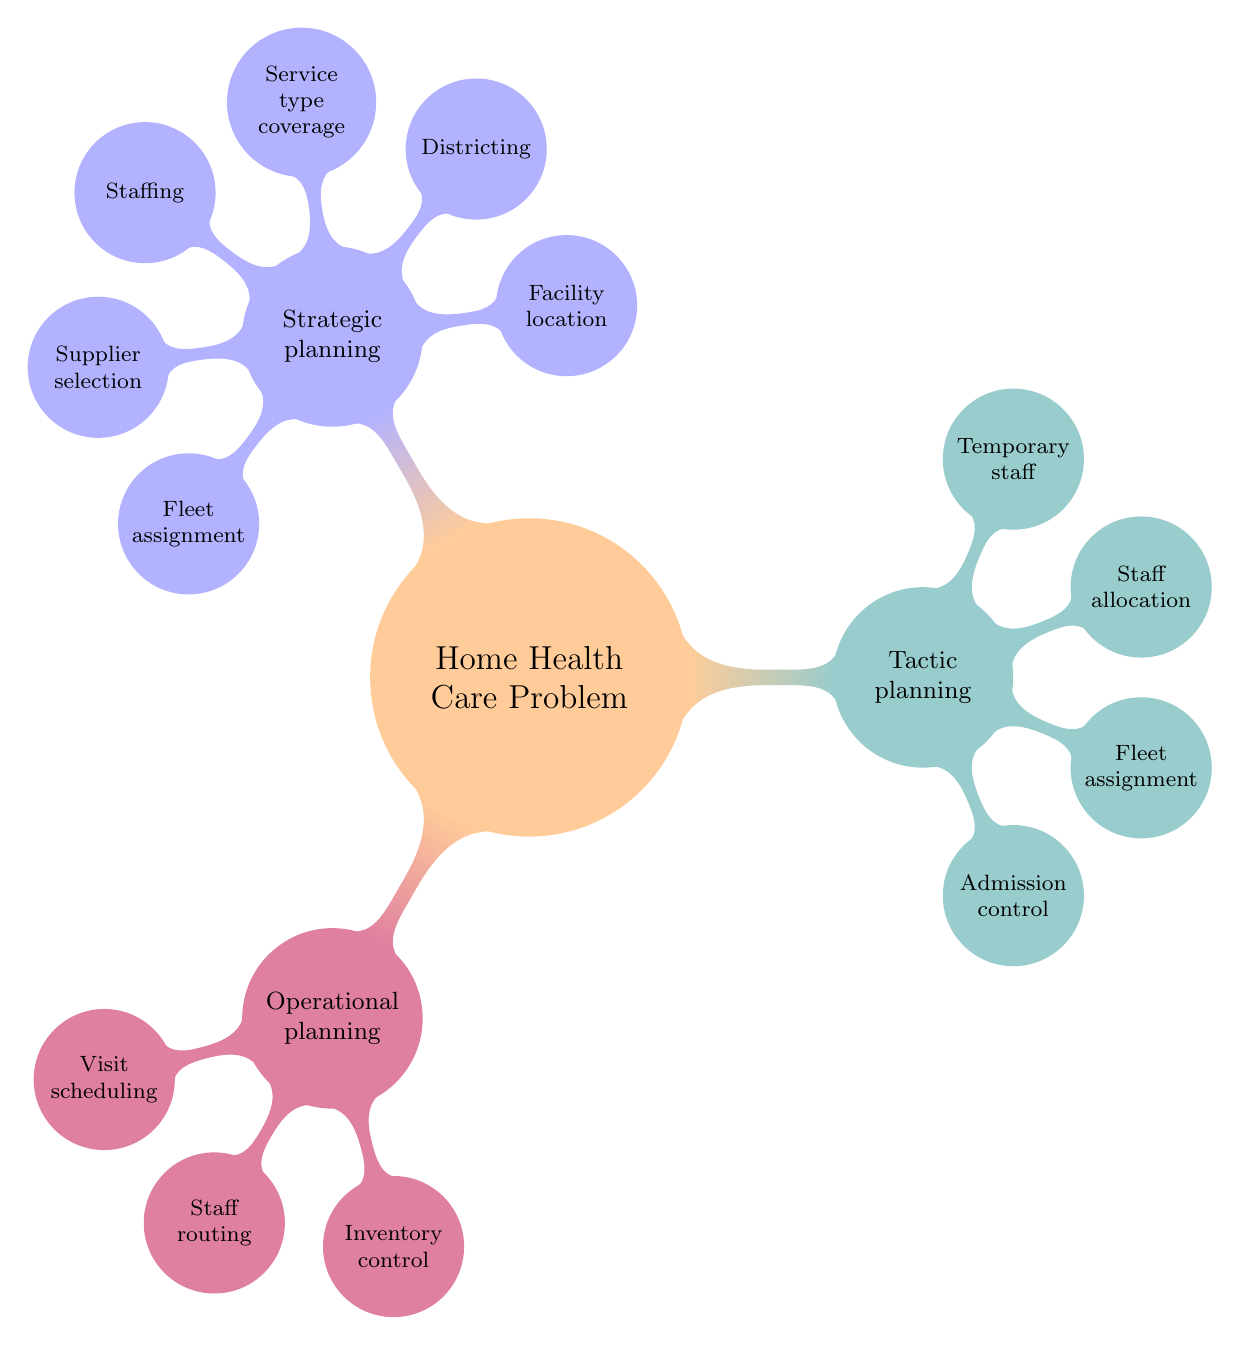
\begin{tikzpicture}[mindmap, grow cyclic, every node/.style=concept, concept color=orange!40,
      level 1/.append style={level distance=5cm,sibling angle=120},
      level 2/.append style={level distance=3cm,sibling angle=45}]

         \node{  Home Health Care Problem}
         child [concept color=purple!50] { node {  Operational planning}
            child { node {Visit scheduling}}
            child { node {Staff routing}}
            child { node {Inventory control}}
         }
         child [concept color=teal!40] { node {  Tactic planning}
            child { node {Admission control}}
            child { node {Fleet assignment}}
            child { node {Staff allocation}}
            child { node {Temporary staff}}
         }
         child [concept color=blue!30] { node { Strategic planning}
            child { node {Facility location}}
            child { node {Districting}}
            child { node {Service type coverage}}
            child { node {Staffing}}
            child { node {Supplier selection}}
            child { node {Fleet assignment}}
         };
      \end{tikzpicture}
      \end{adjustbox}
      \\[2pt]
      \footnotesize
      Source: based on the work of \citet{gutierrez2013}.
   \end{center}
}

\frame{
   \frametitle{Operational planning for the HHCP}

   \textbf{Basic definition as a routing problem}
   \begin{itemize}
%      \item \citet{fernandez1974} studied the problem through statistics
      \item Model introduced by \citet{cheng1998}
%      \item Generalization of vehicle routing problem with time-windows \citep{akjiratikarl2007}
      \item Travel times between all pairs of locations
      \item Service times, patients time-windows
   \end{itemize}

}



\frame{
   \frametitle{Operational planning for the HHCP}

   \textbf{Also a rich research subtopic}
   \footnotesize
   \begin{itemize}
      \item Planning horizon length
      \item Working regulations
      \item {Preferences}
      \item {Uncertainty}
      \item Multiple services types
      \item Multiple visits, operations synchronization
      \item \citet{fikar2017}, \citet{cisse2017}, \citet{grieco2020}
   \end{itemize}
   \normalsize

   \vspace*{12pt}

   \textbf{Integrated approaches}
   \footnotesize
   \begin{itemize}
      \item Fluctuation demands and temporary hiring \citep{eveborn2006}
      \item Fleeting and operational planning \citep{fikar2018}
   \end{itemize}
   \normalsize
}

\section{Problem definition}

\begin{frame}[plain]
   \sectionpage
\end{frame}

\begin{frame}
   \frametitle{Home care in Brazil}

   \textbf{Pilot program ``Better in Home''}
   \begin{itemize}
      \item Program started in 2016
      \item Implemented in some big Brazilian cities
      \item Provides home hospitalization
      %      \item Target population: patients eligible to home hospitalization
   \end{itemize}

   \begin{tikzpicture}[overlay]
   \node (a) at (12.2,0) {
      
\includegraphics[scale=0.2]{fig/melhor-em-casa.png}
   };
   \node [below=1pt of a] {Source: DATASUS (2021)};
   \end{tikzpicture}

\end{frame}

\begin{frame}
   \frametitle{Home care in Brazil}

   \textbf{Motivation: } Solve a real problem in Porto Alegre

%   \vspace{12pt}
%
%   \textbf{Pilot program ``Better in Home''}
   \begin{itemize}

%      \item Motivation: population growth and aging
      \item Opportunity for \textbf{knowledge transfer}
      \item Current approach: manual planning
   \end{itemize}

   \begin{tikzpicture}[overlay]
      \node (a) at (11.6,2) {
         
\includegraphics[scale=0.2]{fig/melhor-em-casa.png}
      };
      \node [below=1pt of a] {Source: DATASUS (2021)};
   \end{tikzpicture}
\end{frame}

\begin{frame}
   \frametitle{Home Care in Porto Alegre}

   \textbf{Current problem and solution approach}
   \begin{itemize}
      \item 19 teams (team = car driver + a skilled physician)
      \item 300 patients visited per week
      \item Most of the \textbf{planning is manual}, daily basis
      \item One experienced caregiver
   \end{itemize}


\end{frame}

\begin{frame}
   \frametitle{Home Care in Porto Alegre}


   \textbf{Three-step manual approach}
   \begin{itemize}
      \item Step 1: chooses the patient of the day
      \item Step 2: assign the patients to the teams
      \item Step 3: individual routing of the teams
      \begin{itemize}
         \item Done by the vehicle drive
         \item Mostly a ``nearest neighbor'' strategy
      \end{itemize}
      \item ``Hope for the best'' strategy
   \end{itemize}

\end{frame}

%\begin{frame}
%   \frametitle{Home Care in Porto Alegre}
%
%   \textbf{The problem is much more complex}
%   \begin{itemize}
%      \item Uncertainty regarding patients $\Rightarrow$ re-scheduling
%      \item Less vehicles available than the number of teams
%      \item Equipment needs to be carried according teams's planning
%%      \item Selection of training medical student
%   \end{itemize}
%\end{frame}

\begin{frame}
   \frametitle{Choosing a target problem}

   \textbf{Our methodology}
   \begin{itemize}
      \item Find a \textit{core} optimization problem
      \item Complex enough
      \begin{itemize}
         \item Valuable for the practitioner
         \item Interesting from the scientific perspective
      \end{itemize}
      \item But not too much constrained/specific
   \end{itemize}

   \vspace*{18pt}
  \pause


   \textbf{Problem of choice: } The Home Health Care Routing \\
   \qquad \qquad \qquad \qquad ~~~~ and Scheduling Problem (HHCRSP)


   \begin{tikzpicture}[overlay]
   \node (a) at (11.8,3) {
      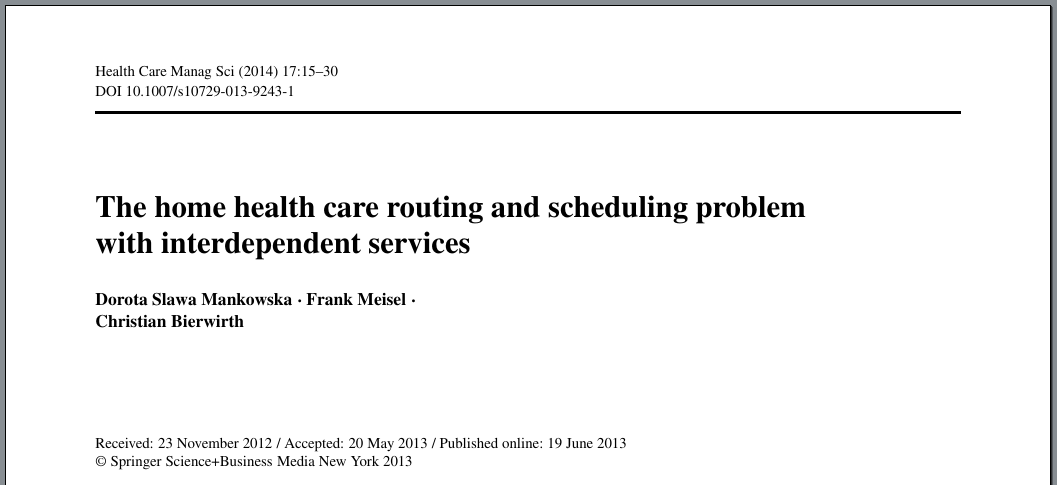
\includegraphics[scale=0.13]{fig/mankowska2014-paper.png}
   };
   \node [below=1pt of a] {\footnotesize \citet{mankowska2014}};
   \end{tikzpicture}

\end{frame}

%\begin{frame}
%   \frametitle{Our target problem}
%
%   \textbf{Some missing characteristics}
%   \begin{itemize}
%      \item Vehicle allocation
%      \item Medical equipment allocation
%      \item Starting point for knowledge transfer
%   \end{itemize}
%\end{frame}

\begin{frame}
   \frametitle{Our target problem}

   \textbf{The home health care routing and scheduling problem}
   \begin{itemize}
%      \item HHCRSP was introduced by \citet{mankowska2014}
      \item Routing (caregivers) and scheduling (visit time)
      \item A model, and heuristics
      \item A public standard benchmark dataset
   \end{itemize}

%   \vspace{20pt}

%   \centering\includegraphics[width=0.9\textwidth]{img/skilled}

\end{frame}


\frame{
   \frametitle{The HHCRSP}

   \textbf{Main characteristics}
   \begin{enumerate}
      \item Routing components
      \item Patient time-window
      \item Covered service types
      \item \onlyh{2}{InfRed}{Operations synchronization on multiple visits}
   \end{enumerate}
}

%
%
%\begin{frame}
%   \frametitle{The HHCRSP: domain features}
%   \textbf{Operations synchronization on double service patients}
%   \begin{itemize}
%      \item Special requirement for patients requiring two service types
%      \item Services must start simultaneously in some patients
%      \item Others have precedence constraints
%      \item Common feature container allocation/transshipment problems \citep{drexl2012synchronization}
%   \end{itemize}
%
%%   \vspace*{8pt}
%
%   \begin{figure}[H]
%      \includegraphics[width=1\textwidth,page=2]{fig/skilled}
%   \end{figure}
%
%\end{frame}

%\frame{
%   \frametitle{The HHCRSP}
%   \textbf{Multiple visit operations synchronization}
%   \begin{itemize}
%      \item Simultaneous attendance
%      \item Precedence constraints + separation time window
%   \end{itemize}
%
%   \begin{figure}[H]
%      \includegraphics[width=1\textwidth,page=2]{fig/skilled}
%   \end{figure}
%
%}

\begin{frame}
   \frametitle{The HHCRSP: Own characteristics}
   \textbf{Double service: precedence order}
   \begin{itemize}
      \item Service precedence: 2 > 5
      \item ($\delta^\mathrm{min}$) and ($\delta^\mathrm{max}$): separation time
   \end{itemize}

   \begin{figure}
      \centering
      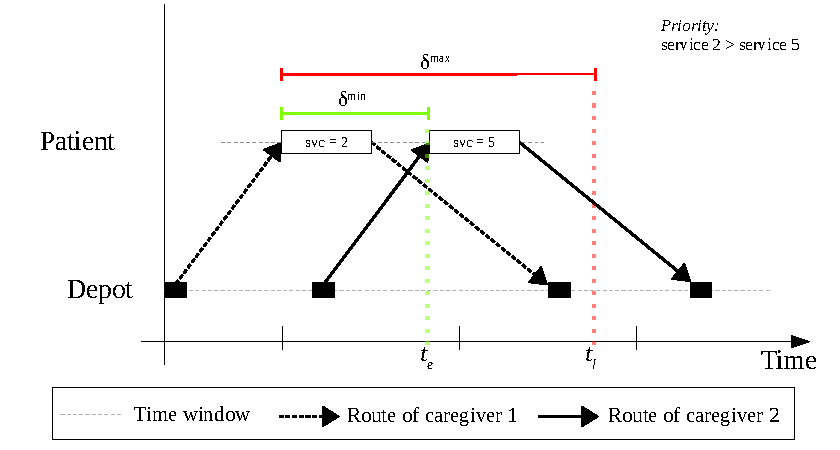
\includegraphics[width=0.6\textwidth,page=1]{fig/sync-tsn2}
   \end{figure}
\end{frame}

\begin{frame}
   \frametitle{The HHCRSP: Own characteristics}
   \textbf{Double service: parallel attendance}
   \begin{itemize}
      \item Services must start simultaneously
   \end{itemize}

   \begin{figure}
      \centering
      \includegraphics[width=0.6\textwidth,page=2]{fig/sync-tsn2}
   \end{figure}
\end{frame}

\frame{
   \frametitle{The HHCRSP: some formal definitions}

   \textbf{Objective function}

%   \only<1> {
%      \begin{gather}
%         \mathrm{Minimize~} \lambda_1 D \; +
%         \lambda_2 T \; +
%         \lambda_3 T^\mathit{max} \nonumber
%      \end{gather}
%   }

%   \only<1> {
      \begin{gather}
      \mathrm{Minimize~}\color{InfRed} \lambda_1 \normalcolor D \; +
      \color{green} \lambda_2 \normalcolor T \; +
      \color{blue} \lambda_3 \normalcolor T^\mathit{max} \nonumber
      \end{gather}
%   }

   \vspace*{12pt}

   \textbf{Components}
   \begin{itemize}
      \item $D$: Sum of traveled distance
      \item $T$: Sum of tardiness
      \item $T^\mathrm{max}$: Maximum tardiness
   \end{itemize}

%   \begin{tikzpicture}[overlay]
%      \draw<3>[InfRed,line width=2pt] (4.3,3.4) rectangle +(0.9, 0.7);
%      \draw<3>[InfRed,line width=2pt] (-0.4, 1.54) rectangle +(6.4, 0.7);
%      \draw<4>[InfRed,line width=2pt] (5.55,3.4) rectangle +(0.9, 0.7);
%      \draw<4>[InfRed,line width=2pt] (-0.4, 0.95) rectangle +(6.4, 0.7);
%      \draw<5>[InfRed,line width=2pt] (6.85, 3.4) rectangle +(1.3, 0.7);
%      \draw<5>[InfRed,line width=2pt] (-0.4, 0.35) rectangle +(6.4, 0.7);
%   \end{tikzpicture}
}


\section{Proposed methods}

\begin{frame}[plain]
   \sectionpage
\end{frame}

%\frame{
%   \frametitle{From the literature}
%
%   \textbf{\citet{mankowska2014}}
%   \begin{itemize}
%      \item MIP model
%      \item VNS-based meta-heuristic (deterministic moves)
%   \end{itemize}
%
%   \vspace*{32pt}
%
%   \textbf{\citet{lasfargeas2019}}
%   \begin{itemize}
%      \item Several variations of a constructive heuristic
%      \item VNS-based meta-heuristic (randomized moves)
%   \end{itemize}
%
%   \begin{tikzpicture}[overlay]
%      \node at (12,4) {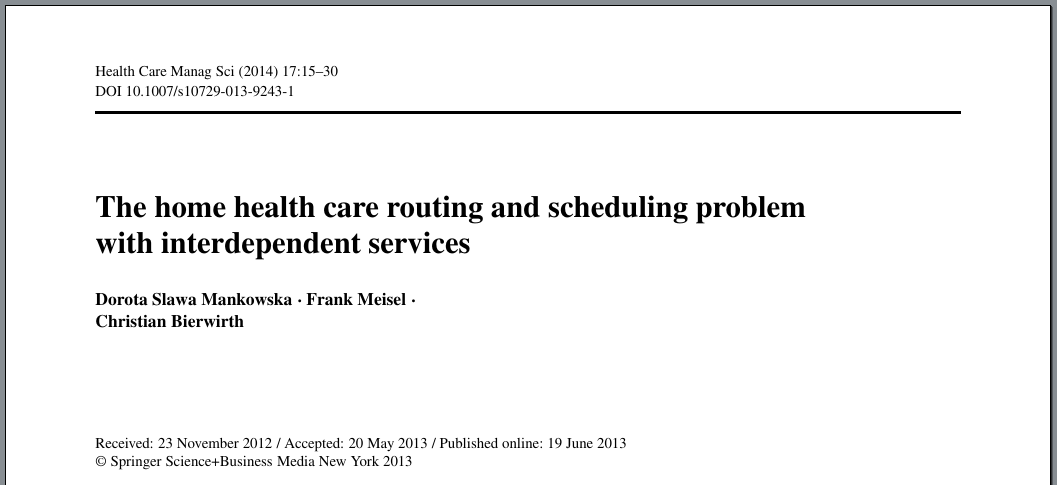
\includegraphics[scale=0.13]{fig/mankowska2014-paper.png}};
%      \node at (12,1) {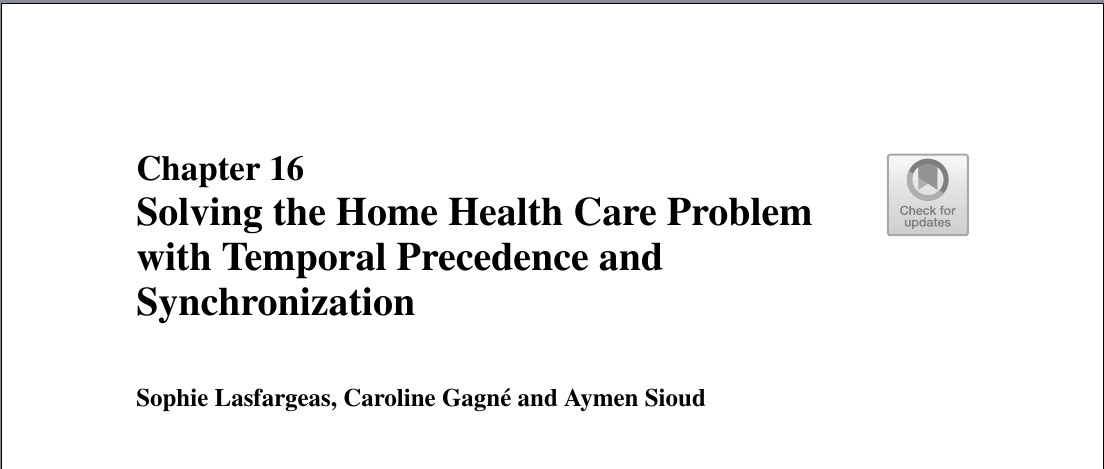
\includegraphics[scale=0.12]{fig/lasfargeas2019-paper.png}};
%   \end{tikzpicture}
%}

%\frame{
%   \frametitle{MIP-based methods}
%
%   \textbf{Lower bounds with CPLEX}
%   \begin{itemize}
%      \item In \citet{mankowska2014}: CPLEX 12.3 --- June, 2011
%      \item Our experiment: CPLEX 20.1 --- December, 2020
%      \begin{itemize}
%         \item Pre-processing
%         \item Parameter setting
%         \item MIP warmstart
%      \end{itemize}
%   \end{itemize}
%}

\frame{
   \frametitle{MIP-based methods}

   \textbf{Fix and optimize matheuristic}
   \begin{itemize}
      \item Initial solution: constructive heuristic \citep{mankowska2014}
      \item Each iteration: optimizes pair of routes
      \item Stop criteria: \# iterations without improvement
   \end{itemize}

   \vspace{12pt}

   \centering
   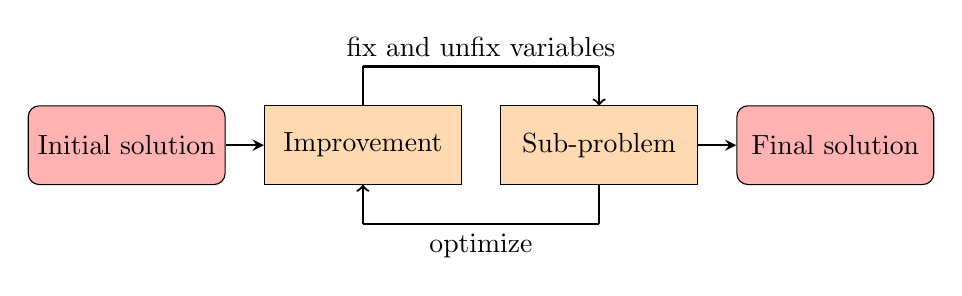
\begin{tikzpicture}[node distance=3cm]
%      \begin{adjustbox}{width=0.02\textwidth}
      \tikzstyle{startstop} = [rectangle, rounded corners, minimum width=2.5cm, minimum height=1cm,text centered, draw=black, fill=red!30]
      \tikzstyle{process} = [rectangle, minimum width=2.5cm, minimum height=1cm, text centered, draw=black, fill=orange!30]
      \tikzstyle{arrow} = [thick,->,>=stealth]

      \node (start) [startstop] {Initial solution};
      \node (pro1) [process, right of=start] {Improvement};
      \node (pro2) [process, right of=pro1] {Sub-problem};
      \node (end) [startstop, right of=pro2] {Final solution};

      \draw [arrow] (start) -- (pro1);
      \draw [arrow] (pro2) -- (end);


      \draw[thick,-] (3,1) -- (6,1) node [pos=0.5, above] {fix and unfix variables};
      \draw[thick,->] (6,1) -- (6,.5);
      \draw[thick,-] (3,1) -- (3,.5);

      \draw[thick,-] (3,-1) -- (6,-1) node [pos=0.5, below] {optimize};
      \draw[thick,-] (6,-1) -- (6,-.5);
      \draw[thick,->] (3,-1) -- (3,-.5);
%      \end{adjustbox}
   \end{tikzpicture}
}

\frame{
   \frametitle{Indirect search methods}

   \textbf{Local search-based methods can be expensive}
   \begin{itemize}
      \item Tricks from VRPTW literature reduce effort of evaluating moves
      \item But the synchronization constraints are too impacting
      \item Requires updating large chunks of the solution
   \end{itemize}

   \vspace*{18pt}

   \textbf{Our proposal:} indirect search \citep{drexl2012}
}


\frame{
   \frametitle{Indirect search methods}

   \textbf{BRKGA}
   \begin{itemize}
      \item Main concept by \citet{bean1994}
      \item Most popular version by \citet{gonccalves2011art}
   \end{itemize}

   \vspace*{18pt}

   \textbf{Intensification components (BRKGA-IC)}
   \begin{itemize}
      \item Island model (also in \citet{toso2015})
      \item Multi-parent mating
      \item Implicit path relinking on random keys space
      \item Proposed by \citet{andrade2021}
   \end{itemize}

   \begin{tikzpicture}[overlay]
      \node at (11.6,1.8) {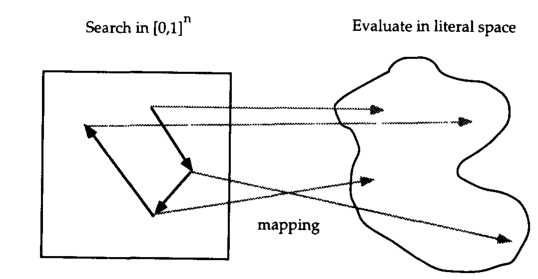
\includegraphics[scale=0.6]{fig/bean1994-rkga-decode.pdf}};
   \end{tikzpicture}
}

%\frame{
%   \frametitle{Indirect search methods}
%
%   \textbf{For the home health care problem}
%   \begin{itemize}
%      \item BRKGA $\Rightarrow$ gives a \textit{permutation} of the patients/nodes
%%      \item The proposed decoder \textit{embeds} a greedy heuristic
%      \item A \emph{best-insertion heuristic decoder} builds a routing solution from the permutation
%   \end{itemize}
%
%%   \vspace*{12pt}
%
%%   \textbf{In short:} TAS $\approx$ permutation of nodes
%
%
%
%%   \begin{figure}
%%      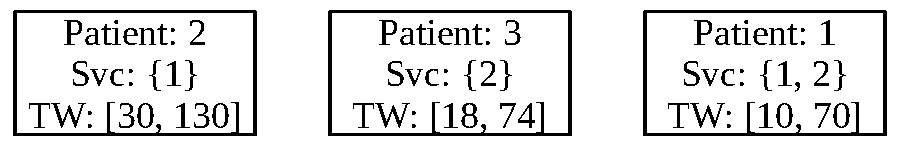
\includegraphics[width=0.5\textwidth]{fig/decoder-tis}
%%   \end{figure}
%}



\section{Preliminary results}

\begin{frame}[plain]
   \sectionpage
\end{frame}


\frame{
   \frametitle{Instance datasets}

   \textbf{\citet{mankowska2014} dataset}
   \begin{itemize}
      \item Total of 70 instances available
      \item Seven instance subsets, from A to G
      \item Euclidean distances
      \item Time-windows of 2 hours % within a 10 hour planning horizon
   \end{itemize}

   \vspace*{12pt}

   \textbf{Service types}
   \begin{itemize}
      \item Fixed $\Sk = \{1, 2, 3, 4, 5, 6\}$
      \item A caregiver can perform up to 3 service types
      \item 70\% of single service patients
      \item 30\% of double services
   \end{itemize}
}

\frame{
   \frametitle{Instance datasets}

   \textbf{\citet{mankowska2014} dataset}

   \begin{table}[H]
      \centering
      \footnotesize
      \begin{tabular}{lrrrrr}
         \toprule
         Instance subset & $|\mathcal{V}|$ & $|\mathcal{C}|$ &
         Avg. cols$^*$ \\
         \toprule
         A &  3 &  10 &      2,445 \\
         B &  5 &  25 &     21,219 \\
         C & 10 &  50 &    159,429 \\
         D & 15 &  75 &    527,139 \\
         E & 20 & 100 &  1,236,846 \\
         F & 30 & 200 &  7,309,566 \\
         G & 40 & 300 & 21,818,286 \\
         \midrule
         \multicolumn{4}{c}{Total of instances: 70}\\
         \bottomrule
      \end{tabular}
   \end{table}

   \vspace*{12pt}

   Ten instances for each subset.

%   $^*$With preprocessing to skip generation of variables trivially set to 0.
}

\frame{
   \frametitle{Instance datasets}

   \textbf{New realistic benchmark dataset}
   \begin{itemize}
      \item Considering the characteristics of Porto Alegre
      \item Realistic patient locations with OpenAddresses database
      \item Realistic travel times with OpenStreetMaps and OpenSourceRoutingMachine
      \item Modified version of \texttt{ovig} tool \citep{sartori2020-pdptw}
   \end{itemize}
}

\frame{
   \frametitle{Instance datasets}

   \textbf{New realistic benchmark dataset}
   \begin{itemize}
      \item Similar to \citep{mankowska2014} dataset
      \item Demands proportional to the available qualified manpower
      \item Can be easily extended to generate weekly instances
   \end{itemize}

   \begin{table}[H]
      \footnotesize
      \begin{tabular}{lrr}
         \toprule
         Instance subset & $|\mathcal{V}|$ & $|\mathcal{C}|$\\
         \midrule
         A & 10 & 3\\
         B & 25 & 4\\
         C & 75 & 12\\
         D & 100 & 16\\
         E & 200 & 33\\
         F & 300 & 50\\
         G & 500 & 83\\
         H & 700 & 116\\
         I & 850 & 141\\
         J & 1000 & 166\\
         \bottomrule
      \end{tabular}
   \end{table}
}


%\frame{
%   \frametitle{Benchmark machine}
%
%   \textbf{With the F\&O \textit{matheuristic}, and BRKGA}
%   \begin{itemize}
%      \item CPLEX 12.9
%      \item Intel Core i7 3612QM at 3.1 GHz
%      \item 8 GB of memory
%      \item Single thread processing
%   \end{itemize}
%
%   \vspace*{12pt}
%
%   \textbf{With the BRKGA-MP-IPR, and LB$^+$ experiment}
%   \begin{itemize}
%      \item CPLEX 20.10
%      \item Intel Core i7 930 at 2.8 GHz
%      \item 12 GB of memory
%      \item Single thread processing (CPLEX)
%      \item Parallel decoding with 4 threads (BRKGA)
%   \end{itemize}
%}

%\frame{
%   \frametitle{Previous results from the literature}
%
%   \textbf{MIP and MH \citep{mankowska2014}}
%   \begin{itemize}
%      \item CPLEX (mostly) for providing lower bounds
%      \item Initial solutions: nearest neighbor heuristic
%      \item Solution structure: three-indexed matrix
%      \item LS operators: (inter, intra)-route $\times$ (swap, shift)
%      \item Specialized operators for single and double services
%      \item Simple LS, and the Adaptive VNS
%      \item \textit{Best improvement} with a MN heuristic
%      \item \textit{Best improvement} in adaptive phase of VNS
%   \end{itemize}
%}
%
%\frame{
%   \frametitle{Previous results from the literature}
%
%   \textbf{Meta-heuristics \citet{lasfargeas2019}}
%   \begin{itemize}
%      \item Originally proposed for the short-term HHCP
%      \item Several variations of the constructive heuristic
%      \item Repeated construction with randomization
%      \item Operators: equivalent to shif and swap operators from \citet{mankowska2014}, but only single service operators
%      \item Randomizes the choice of patients to shift/swap
%      \item But the operator order is also fixed
%      \item \textit{First improvement} is used within the VNS algorithm
%      \item Results for instances with up to 75 patients
%   \end{itemize}
%}

\frame{
   \frametitle{\footnotesize Previous results from the literature}

   \textbf{MIP and MH \citep{mankowska2014}}
   \begin{itemize}
      \item CPLEX (mostly) for providing lower bounds
      \item Several LS-based heuristics, and a VNS-based algorithm
      \item Specialized operators for single and double services
%      \item Nearest neighbor-like constructive heuristic
   \end{itemize}
}

\frame{
   \frametitle{\footnotesize Previous results from the literature}

   \textbf{Meta-heuristics of \citet{lasfargeas2019}}
   \begin{itemize}
%      \item Repeated construction with randomization
      \item VNS-based metaheuristic
      \item Similar operators than \citet{mankowska2014}
      \item Randomizes the choice of patients to shift/swap
%      \item \textit{First improvement} acceptance
%      \item Results for instances with up to 75 patients
   \end{itemize}
}

%\frame{
%   \frametitle{Environmental setup}
%
%   \textbf{Speed factor between machines}
%   \begin{itemize}
%      \item Too many experiments to replicate
%      \item Many implementation details left off
%      \item Alternative approach: use published results
%      \item But we first need to estimate the speed factor among the distinct benchmark machines
%   \end{itemize}
%
%   \vspace*{12pt}
%
%   \begin{table}[H]
%      \centering
%      \scriptsize
%      \setlength{\tabcolsep}{2.5pt}
%      \renewcommand{\arraystretch}{1.1}
%      \begin{tabular}{llrr}
%         \toprule
%         Publication & Machine description & PassMark score & Factor\\
%         \midrule
%         \citet{mankowska2014} & Intel Core at 3.40 GHz & 1884 & 1.4270\\
%         \citet{lasfargeas2019} & Intel i7 at 4.00 GHz & 2528 & 1.9750\\
%         F\&O & Intel i7-3612QM at 3.10 GHz & 1484 & 1.1559\\
%         BRKGA & Intel i7-3612QM at 3.10 GHz & 1484 & 1.1559\\
%         BRKGA-MP-IPR & Intel i7-930 at 2.80 GHz & 1280 & 1.0000\\
%         \bottomrule
%      \end{tabular}
%   \end{table}
%}

\frame{
   \frametitle{Outline}

   \begin{enumerate}
      \item \onlyh{2}{InfRed}{New lower bounds with CPLEX 20.10}
      \item New upper bounds from BRKGA and BRKGA-MP-IPR
      \item Comparison with the literature
      \item New upper bounds with the MIP
   \end{enumerate}
}

\frame{
   \frametitle{New lower bounds with CPLEX 20.10}

   \bgroup
   \begin{table}[!htb]
      \scriptsize
      \setlength{\tabcolsep}{2.5pt}
      \renewcommand{\arraystretch}{1.1}
      \centering
      \begin{tabular}{lrrrrrr}
         \toprule
         \multirow{2}[2]{*}{Instance} &
         \multicolumn{2}{c}{Previous values} &
         \multicolumn{4}{c}{New values} \\

         \cmidrule(l){2-3}
         \cmidrule(l){4-7}

         & LB$^+$ & Time (sec.)
         & LB$^+$ & Time (sec.) & Improv. (\%)
         & \# Nodes \\
         \midrule

         A & \textbf{225.2} & 5.2 & \textbf{225.2} & 1.0 & 0.0 & 846 \\
         B & 343.1 & 36,000.0 & \textbf{386.0} & 4408.2 & 13.3 & 1,129,013 \\
         C & 342.6 & 36,000.0 & \textbf{403.5} & 7200.0 & 17.7 & 48,480  \\
         D & 377.4 & 36,000.0 & \textbf{411.7} & 7200.0 & 9.0 & 5,808  \\
         E & 404.5 & 36,000.0 & \textbf{418.1} & 7200.0 & 3.4 & 654   \\
         \midrule
         F & 435.3 & 36,000.0 & \textbf{528.6} & 7200.2 & 21.9 & 507   \\
         G & 462.1 & 36,000.0 & \textbf{604.3} & 7200.6 & 30.8 & 302  \\
         \midrule
         & 370.0 & 30857.9 & 425.4 & 5772.9 & 13.7 & 169372.8\\
         \bottomrule
      \end{tabular}
   \end{table}
   \egroup

   \vspace*{12pt}

   Initial solutions from BRKGA \citep{kummer2020}.
}

\frame{
   \frametitle{Outline}

   \begin{enumerate}
      \item \onlyh{1}{InfRed}{New lower bounds with CPLEX 20.10}
      \item \onlyh{2,3}{InfRed}{New upper bounds from BRKGA and BRKGA-MP-IPR}
      \only<2->{
      \begin{enumerate}
         \item \onlyh{3}{InfRed}{Automatic algorithm configuration}
         \item Computational results
      \end{enumerate}
      }
      \item Comparison with the literature
      \item New upper bounds with the MIP
   \end{enumerate}
}


\frame{
   \frametitle{Calibrating the BRKGA}

   \textbf{Highly parameterized heuristics}
   \begin{itemize}
      \item BRKGA has five parameters
      \item Island models: +3
      \item New parameters for MP: +3
      \item IPR: +5
      \item Stagnated generations before reset +1

      \item \textbf{Total: 17 parameters}
   \end{itemize}
}

\frame{
   \frametitle{Calibrating the BRKGA}

   \textbf{Automatic algorithm configuration with \emph{irace}}
   \begin{itemize}
      \item R package, easy to use \emph{front-end}
      \item Stopping criteria $\Rightarrow$ \emph{budget}, or time limit
      \item A parameter space specification
%      \item Rules for forbidden configurations
      \item A set of train instances
   \end{itemize}

   \vspace*{12pt}

   \textbf{Advantages over manual configuration}
   \begin{itemize}
      \item Prevent human errors and bias
      \item Robust experiment
   \end{itemize}

   \color{InfRed} Starting point for newcomers: \citet{lopez2016} for irace guidance, \citet{eggensperger2019-aac-best-practices} for general advice
}

%\frame{
%   \frametitle{Calibrating the BRKGA}
%
%   \textbf{\emph{irace} for BRKGA}
%   \begin{itemize}
%      \item Parameters: 5
%      \item Budget: 5,000 runs
%      \item Train instances: C subset (50 patients, 10 caregivers)
%      \item Total time spent: $\approx{}$ 3 days
%   \end{itemize}
%
%   \vspace*{12pt}
%
%   \textbf{\emph{irace} for BRKGA-MP-IPR}
%   \begin{itemize}
%      \item Parameters: 17
%      \item Budget: 1,500 runs
%      \item Train instances: G subset (300 patients, 40 caregivers)
%      \item Total time spent: $\approx{}$ 3 days
%   \end{itemize}
%}

\frame{
   \frametitle{Outline}

   \begin{enumerate}
      \item New lower bounds with CPLEX 20.10
      \item \onlyh{1-}{InfRed}{New upper bounds from BRKGA and BRKGA-MP-IPR}
      \begin{enumerate}
         \item \onlyh{1}{InfRed}{Automatic algorithm configuration}
         \item \onlyh{2}{InfRed}{Computational results}
      \end{enumerate}
      \item Comparison with the literature
      \item New upper bounds with the MIP
   \end{enumerate}
}


\frame{
   \frametitle{Comparison of results}

   \begin{itemize}
      \item 15 runs for each instance
%      \item BRKGA: \citep{kummer2020}
%      \item BRKGA-MP-IPR: ongoing write
   \end{itemize}

   \begin{table}[H]
      \tiny
      \centering
      \setlength{\tabcolsep}{3pt}
      \begin{tabular}{lrrrrrrrr}
         \toprule

         \multirow{2}[2]{*}{Instance} &
         \multirow{2}[2]{*}{LB$^+$} &
         \multicolumn{3}{c}{BRKGA} &
         \multicolumn{4}{c}{BRKGA-MP-IPR}\\

         \cmidrule(lr){3-5}
         \cmidrule(lr){6-9}

         & &
         Cost & Gap (\%) & Time (sec) &
         Cost & Gap (\%) & Improv. (\%) & Time (sec)\\



         \midrule


         A & 225.2 & \textbf{227.5} & \textbf{1.0} & 2.7 & \textbf{227.5} & \textbf{1.0} & 0.0 & 97.7 \\
         B & 386.0 & \textbf{413.9} & \textbf{6.7} & 10.3 & \textbf{413.9} & \textbf{6.7} & 0.0 & 105.4 \\
         C & 403.5 & 629.1 & 35.9 & 43.5 & \textbf{627.0} & \textbf{35.6} & -0.4 & 130.7 \\
         D & 411.7 & 792.2 & 48.0 & 109.6 & \textbf{783.9} & \textbf{47.5} & -1.1 & 165.9 \\
         E & 418.1 & 846.1 & 50.6 & 211.3 & \textbf{829.0} & \textbf{49.6} & -2.0 & 219.8 \\
         F & 528.6 & 1278.1 & 58.6 & 899.6 & \textbf{1232.3} & \textbf{57.1} & -3.6 & 577.2 \\
         G & 604.3 & 1709.7 & 64.7 & 2214.0 & \textbf{1632.7} & \textbf{63.0} & -4.5 & 1228.5 \\
         \midrule
         & 425.3 & 842.4 & 37.9 & 498.7 & \textbf{820.9} & \textbf{37.2} & -1.7 & 360.7\\
         \bottomrule
      \end{tabular}
   \end{table}
}

\frame{
   \frametitle{Outline}

   \begin{enumerate}
      \item New lower bounds with CPLEX 20.10
      \item \onlyh{1}{InfRed}{New upper bounds from BRKGA and BRKGA-MP-IPR}
      \begin{enumerate}
         \item Automatic algorithm configuration
         \item \onlyh{1}{InfRed}{Computational results}
      \end{enumerate}
      \item \onlyh{2}{InfRed}{Comparison with the literature}
      \item New upper bounds with the MIP
   \end{enumerate}
}

\frame{
   \frametitle{Comparison of results}

   \begin{itemize}
      \item Fix and Optimize: single run
%      \item BRKGA-MP-IPR: 15 runs
   \end{itemize}

\begin{table}[H]
   \tiny
   \setlength{\tabcolsep}{3pt}
%   \renewcommand{\arraystretch}{1.13}
   \begin{tabular}{lrrrrrrrrrrrrrrrrrr}


      \toprule
      \multirow{2}[2]{*}{Instance} &
      \multirow{2}[2]{*}{LB$^+$} &
      \multicolumn{3}{c}{MK} &
      \multicolumn{3}{c}{LF} &
      \multicolumn{3}{c}{F\&O} &
      \multicolumn{3}{c}{BRKGA-MP-IPR}
      \\

      \cmidrule(lr){3-5}
      \cmidrule(lr){6-8}
      \cmidrule(lr){9-11}
      \cmidrule(lr){12-14}

      & & Cost  & Gap & Time
      & Cost & Gap &   Time
      & Cost & Gap  & Time
      & Cost  & Gap &  Time
      \\
      \midrule

      A& 225.2 & \textbf{225.2} & 0.0 &  7.7 & \textbf{225.2} & 0.0  &  1.0 & \textbf{225.2} & 0.0 & 0.5 & 227.5 & 1.0  & 97.7 \\

      B& 386.0 & 445.4 & 13.3 &  26,494.3 & \textbf{411.2} & 6.1 &  94.8 & 426.5 & 9.5 & 102.2 & 413.9 & 6.7 &  105.4 \\

      C& 403.5 & 713.2 & 43.4 &  1.0 & 636.2 & 36.6 &  215.3 & 646.3 & 37.6 & 475.6 & \textbf{627.0} & 35.6 & 130.7 \\

      D& 411.7 & 928.6 & 55.7 &  6.8 & 854.0 & 51.8 &  309.6 & 853.0 & 51.7 & 1113.3 & \textbf{783.9} & 47.5 &165.9 \\

      E& 418.1 & 1057.6 & 60.5 &  24.4 & -- & -- &  -- & 966.1 & 56.7 & 4101.3 & \textbf{829.0} & 49.6 & 219.8 \\

      F& 528.6 & 1588.0 & 66.7 &  1641.7 & -- & -- &   -- & -- & -- & -- & \textbf{1232.3} & 57.1 & 577.2 \\

      G& 604.3 & 2161.2 & 72.0 &  10,495.5 & -- & -- &   -- & -- & -- & -- & \textbf{1632.7} & 63.0 &  1228.5 \\

      \midrule
      & 425.3 & 1017.0 & 44.5 & 5524.5 & 531.7 & 23.6 & 155.2 & 623.4 & 31.1 & 1158.6 & 820.9 & 37.2 & 360.7\\

      \bottomrule
   \end{tabular}
\end{table}
}

\frame{
   \frametitle{Outline}

   \begin{enumerate}
      \item New lower bounds with CPLEX 20.10
      \item New upper bounds from BRKGA and BRKGA-MP-IPR
      \begin{enumerate}
         \item Automatic algorithm configuration
         \item Computational results
      \end{enumerate}
      \item \onlyh{1}{InfRed}{Comparison with the literature}
      \item \onlyh{2}{InfRed}{New upper bounds with the MIP}
   \end{enumerate}
}


\frame{
   \frametitle{Comparison of results}

   \textbf{New upper bounds while LB$^+$ experiment}
   \begin{itemize}
      \item New BKV for 9 instances from subset B
      \item New BKV for all instances from subset C
      \item New BKV for 3 instances from subset D
   \end{itemize}

   \begin{table}[H]

      \centering
      \footnotesize
      \begin{tabular}{lrrrrr}
         \toprule
         \multirow{2}[1]{*}{Instance } &
         \multicolumn{5}{c}{Optimal solutions} \\
         \cmidrule{2-6}

         & LB$^+$ & Initial (obj) & Final (obj) & Time (sec.) & Gap (\%)
         \\
         \midrule
         B1 & 428.1 & 428.6 & \textbf{428.1} & 5970.3 & 0.0 \\
         B2 & 476.0 & 483.6 & \textbf{476.0} & 469.5 & 0.0 \\
         B4 & 411.3 & 432.2 & \textbf{411.3} & 509.9 & 0.0 \\
         B7 & 328.6 & 328.7 & \textbf{328.7} & 598.7 & 0.0 \\
         B8 & 357.6 & 359.7 & \textbf{357.7} & 533.7 & 0.0 \\
         \bottomrule
      \end{tabular}
   \end{table}

%   \begin{tikzpicture}[overlay]
%      \node<2>[rectangle, fill=green, anchor=south, text=black] at (5.65,1.2) {\scriptsize $\approx 5.84\%$};
%   \end{tikzpicture}

}



\section{Future works}

\begin{frame}[plain]
   \sectionpage
\end{frame}

\frame{
   \frametitle{Proposed schedule}

   \begin{table}[H]
      \centering
      \scriptsize
      \begin{tabular}{lccccccc}
         \toprule
         Item & Jan & Feb & Mar & Apr & May & Jun & Jul\\
         \midrule
         1. BRKGA for other datasets & & & & x \\
         \midrule
         2. Journal article \\
         \phantom {2.} 2.1 BRKGA-MP-IPR & &x & x & x &  &  & \\
         \phantom {2.} 2.2 SP/MWIS heuristics & & &  & x & x & x &x \\
         \midrule
         3. New lower bounds\\
         \phantom{3. } 3.1 Additional cuts & & & x & x \\
         \phantom{3. } 3.2 VRPSolver & x & & & x & x & x\\
         \midrule
         4. Route recombination heuristics\\
         \phantom{4. } 4.1 With set partitioning & & & x & x & x & x\\
         \phantom{4. } 4.2 With maximum weighted IS & & & x & x & x & x\\
         \midrule
         5. HHCRSP in Porto Alegre\\
         \phantom{5.} 5.1 New instance dataset & x  & & & x & x & x\\
         \phantom{5.} 5.2 Adaption of methods & & & & && x & x \\
         \phantom{5.} 5.3 Simple heuristics  & & & & && x & x \\
         \midrule
         6. Thesis writing & & x & x & x & x & x & x \\
         \bottomrule
      \end{tabular}
   \end{table}
}

\frame{
   \frametitle{Current schedule}

   \begin{table}[H]
      \centering
      \scriptsize
      \begin{tabular}{lccccccc}
         \toprule
         Item & Jan & Feb & Mar & Apr & May & Jun & Jul\\
         \midrule
         \color{InfRed} 1. BRKGA for other datasets & & & & x & \textbf{x} \\
         \midrule
         \color{InfRed} 2. Journal article \\
         \color{InfRed} \phantom {2.} 2.1 BRKGA-MP-IPR & &x & x & x &  &  & \\
         \phantom {2.} 2.2 SP/MWIS heuristics & & &  & x & x & x &x \\
         \midrule
         3. New lower bounds\\
         \phantom{3. } \sout{3.1 Additional cuts} & & & x & x \\
         \color{InfRed} \phantom{3. } 3.2 VRPSolver & x & & & x & x & x\\
         \midrule
         \color{InfRed} 4. Route recombination heuristics\\
         \color{InfRed} \phantom{4. } 4.1 With set partitioning & & & x & x & x & x\\
         \color{InfRed} \phantom{4. } 4.2 With maximum weighted IS & & & x & x & x & x\\
         \midrule
         5. HHCRSP in Porto Alegre\\
         \color{InfRed} \phantom{5.} 5.1 New instance dataset & x  & & & x & x & x\\
         \phantom{5.} 5.2 Adaption of methods & & & & && x & x \\
         \phantom{5.} 5.3 Simple heuristics  & & & & && x & x \\
         \midrule
         \color{InfRed} 6. Thesis writing & & x & x & x & x & x & x \\
         \bottomrule
      \end{tabular}
   \end{table}
}

\frame{
   \frametitle{Current schedule}

   \textbf{2.1 BRKGA-MP-IPR}
   \begin{itemize}
      \item Article is almost finished
      \item Small adjusts in the formatting
   \end{itemize}

   \vspace{12pt}
   \textbf{Estimated completion:} week 18 (May, 7)
}

\frame{
   \frametitle{Current schedule}

   \textbf{1. BRKGA for other datasets}
   \begin{itemize}
      \item Additional instance features
      \item Dataset from \citet{bredstrom2008}
      \item Dataset from \citet{rasmussen2012}
   \end{itemize}

   \vspace{12pt}
   \textbf{Estimated completion:} week 19 (May, 14)
}

\frame{
   \frametitle{Current schedule}

   \textbf{3.2 VRPSolver}
   \begin{itemize}
      \item A Branch-and-Cut-and-Price based exact solver for routing-like problems
      \item Proposed by \citet{pessoa2020}
      \item Can be used as a Julia library
   \end{itemize}

   \vspace{12pt}
   \textbf{Estimated completion:} week 21 (May, 28)
   \begin{itemize}
      \item $\approx$ 70\% done
      \item \onlyh{2}{InfRed}{No support to synchronization constraints}
      \item \onlyh{2}{InfRed}{No support to soft time-windows}
      \item Optimal solutions to the VRPTW: combinatorial lower bounds \citep{uma2006}
   \end{itemize}
}

\frame{
   \frametitle{Current schedule}

   \textbf{4. Route recombination heuristics}\\
   \textbf{2.2 SP/MWIS heuristic paper}
   \begin{itemize}
      \item Try to find improved solutions from a \textit{pool} of routes
      \item Adjustments of visits times (operations synchronization)
   \end{itemize}

   \vspace{12pt}
   \textbf{Estimated completion:} week 21 (May, 28)
   \begin{itemize}
      \item $\approx$ 30\% done
      \item BRKGA $\Rightarrow$ to generate routes
      \item A SP-based model to combine the routes
      \item CPLEX to solve SP
   \end{itemize}
}

\frame{
   \frametitle{Current schedule}

   \textbf{5.1. New instance dataset}
   \begin{itemize}
      \item Porto Alegre does not save historical data of past months of HHC services
      \item Our proposal: generate instances similar to the real ones
      \item Approach similar to \citet{sartori2020-pdptw}
   \end{itemize}

   \vspace{12pt}
   \textbf{Estimated completion:} week 22 (June, 4)
   \begin{itemize}
      \item With the \textit{ovig} library: $\approx$ 50\% done
      \item Pending visit to the operations center of Porto Alegre
      \item Tomorrow: meeting with the software developers responsible for Porto Alegre city hall systems
   \end{itemize}
}

\frame{
   \frametitle{Current schedule}

   \textbf{5.2. Adaption of methods}\\
   \textbf{5.3. Simple heuristics}
   \begin{itemize}
      \item Adapt ou solution methods to the new instance dataset
      \item Propose simple heuristics
      \item \textcolor{InfRed}{Uncertainty}
   \end{itemize}

   \vspace{12pt}
   \textbf{Estimated completion:} week 26 (July, 2)
   \begin{itemize}
      \item Effort depends upon features of the new instance dataset
   \end{itemize}
}

\section{References}

\begin{frame}[plain]
   \sectionpage
\end{frame}

\frame[allowframebreaks]{
   \frametitle{Bibliography}
   \scriptsize
   \setbeamertemplate{bibliography item}[triangle]
   \bibliographystyle{plainnat}
   \bibliography{bibliography}
}

\section*{}

%\begin{frame}
%%    \frametitle{Thank you!}
%   \vspace*{40pt}
%   \InfContacts
%\end{frame}

\begin{frame}
   \frametitle{Thank you!}
   \begin{center}
      \footnotesize
      \textbf{Alberto F. Kummer$^1$, Olinto C.B. de Araújo$^2$,\\Luciana S. Buriol$^{1,4}$, and Mauricio, G.C. Resende$^{3,4}$}

      \vspace*{8pt}

      $^1$Federal University of Rio Grande do Sul\\
      \texttt{\{\textcolor{InfRed}{afkneto},buriol\}@inf.ufrgs.br}
      \vspace*{6pt}

      $^2$Federal University of Santa Maria\\
      \texttt{olinto@ctism.ufsm.br}
      \vspace*{6pt}

      $^3$University of Washington\\
      \texttt{mgcr@berkeley.edu}
      \vspace*{6pt}

      $^4$Amazon.com, Inc.
   \end{center}

\end{frame}

\end{document}
